%!TEX root = ./cikm2016.tex
\begin{figure*}[t]
	\centering
	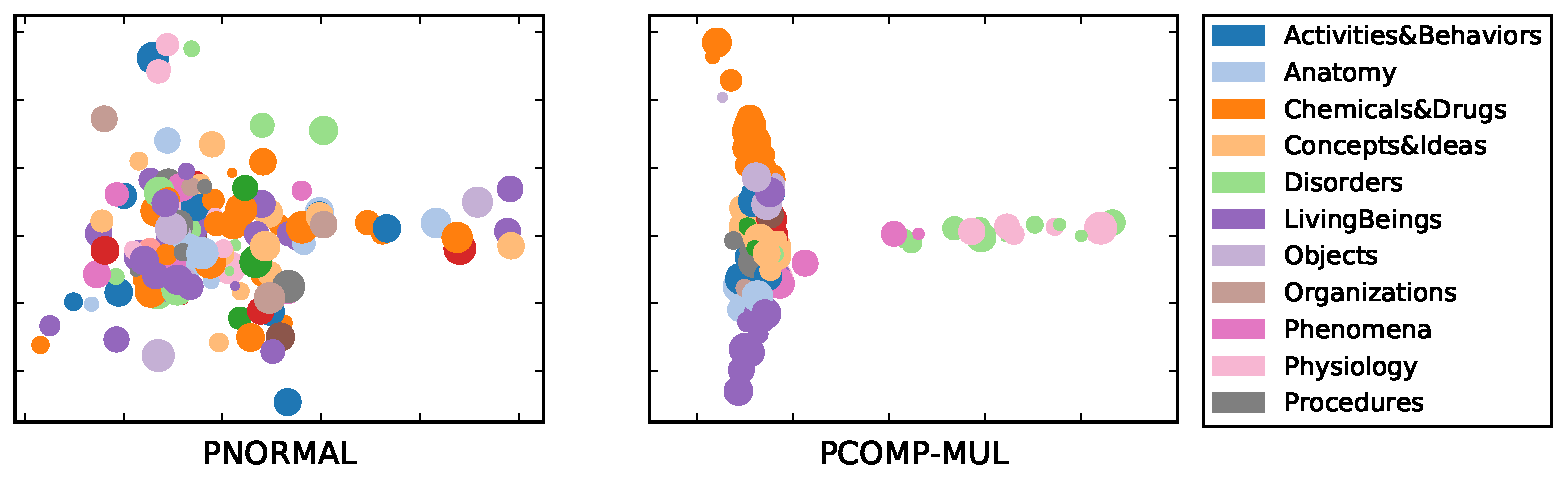
\includegraphics[width=0.7\linewidth]{images/embedding_umls.pdf}
	\caption{\label{fig:tsne} Embedding learned entities of the UMLS dataset into a two-dimensional space through the spectral clustering. Entities with the same type are represented by the same color.}
\end{figure*}

\section{Visualisation}

\label{sec:vis}
In Figure \ref{fig:tsne}, we visualise the multi-dimensional entities inferred by \textsc{Pnormal} and \textsc{Pcomp-mul}
into a two-dimensional space through the spectral clustering \cite{von2007tutorial}.
A circle represents an entity, and the size of the circle is proportional to the uncertainty of the entity in the latent space.
In the UMLS dataset, the entities are categorised into 15 types,
e.g. \texttt{Disorders}, \texttt{Living-Beings}, \texttt{Phenomena}, etc.
We use the same color to represent the entities with the same type.
The entities with the same type are located closer to each other with \textsc{Pcomp-mul} than \textsc{Pnormal}.
